\documentclass[11pt,a4paper]{article}

% These are extra packages that you might need for writing the equations:
\usepackage{amsmath}
\usepackage{amsfonts}
\usepackage{amssymb}
\usepackage{booktabs}
\usepackage{hyperref}
\usepackage{listings}
\usepackage{xcolor}
\usepackage{graphicx}
\usepackage{subfig}
\usepackage{float}

\lstset {language=C++,
		 basicstyle=\ttfamily,
         keywordstyle=\color{blue}\ttfamily,
         stringstyle=\color{red}\ttfamily,
         commentstyle=\color{purple}\ttfamily,
         morecomment=[l][\color{magenta}]{\#},
       	 basicstyle=\tiny}

% You need the following package in order to include figures in your report:
\usepackage{graphicx}

% With this package you can set the size of the margins manually:
\usepackage[left=2cm,right=2cm,top=2cm,bottom=2cm]{geometry}

\begin{document}

% Enter the exercise number, your name and date here:
\noindent\parbox{\linewidth}{
 \parbox{.25\linewidth}{ \large HPCSE I, Exercise 10 }\hfill
 \parbox{.5\linewidth}{\begin{center} \large Beat Hubmann \end{center}}\hfill
 \parbox{.2\linewidth}{\begin{flushright} \large Dec 10, 2018 \end{flushright}}
}
\noindent\rule{\linewidth}{2pt}

\section{Question 1: MPI I/O with a Custom Data Compressor}

\subsection{a) and b)}
Done as instructed and submitted.

\subsection{c)}
The obtained compression rates when varying the compression tolerance from $0$ to $10$ in steps of $0.2$
are shown in figure~\ref{fig:1}. The losslessly zipped input file has a compression ratio of $\frac{134.2\text{MB}}{17.4\text{MB}}\ \approx \ 7.7$.
As figure~\ref{fig:1} shows, any compression tolerance $\ge 0.4$ achieves a similar or higher compression ratio. This is however at
the cost of being lossy by nature due to \texttt{zfp} being a lossy compressor.

\begin{figure}[ht]
\begin{center}
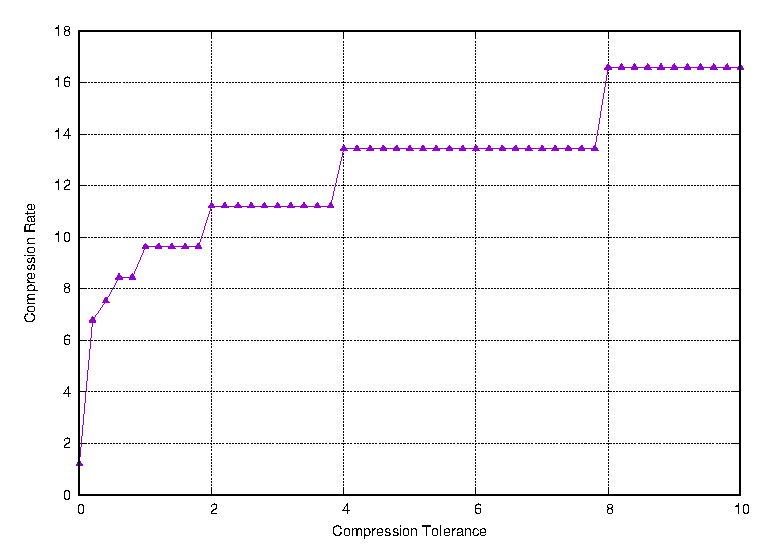
\includegraphics[scale=1.0]{compare.eps} 
\end{center}
\caption{Compression rate vs compression tolerance (number of processes $N=4$).} 
\label{fig:1}
\end{figure}

\section{Question 2: Weak Scaling}

\subsection{a)}

The weak scaling plot for the given data (figure~\ref{fig:2}) and $N=1024,\ p=1$ as baseline reference is shown in figure~\ref{fig:3}.
The plot hints at a weak efficiency of about 85\% ($\lim_{p \rightarrow \infty}\frac{t_1}{t_p} = E_w\ \approx\ 0.85$).



\begin{figure}[ht!]
    \begin{center}
    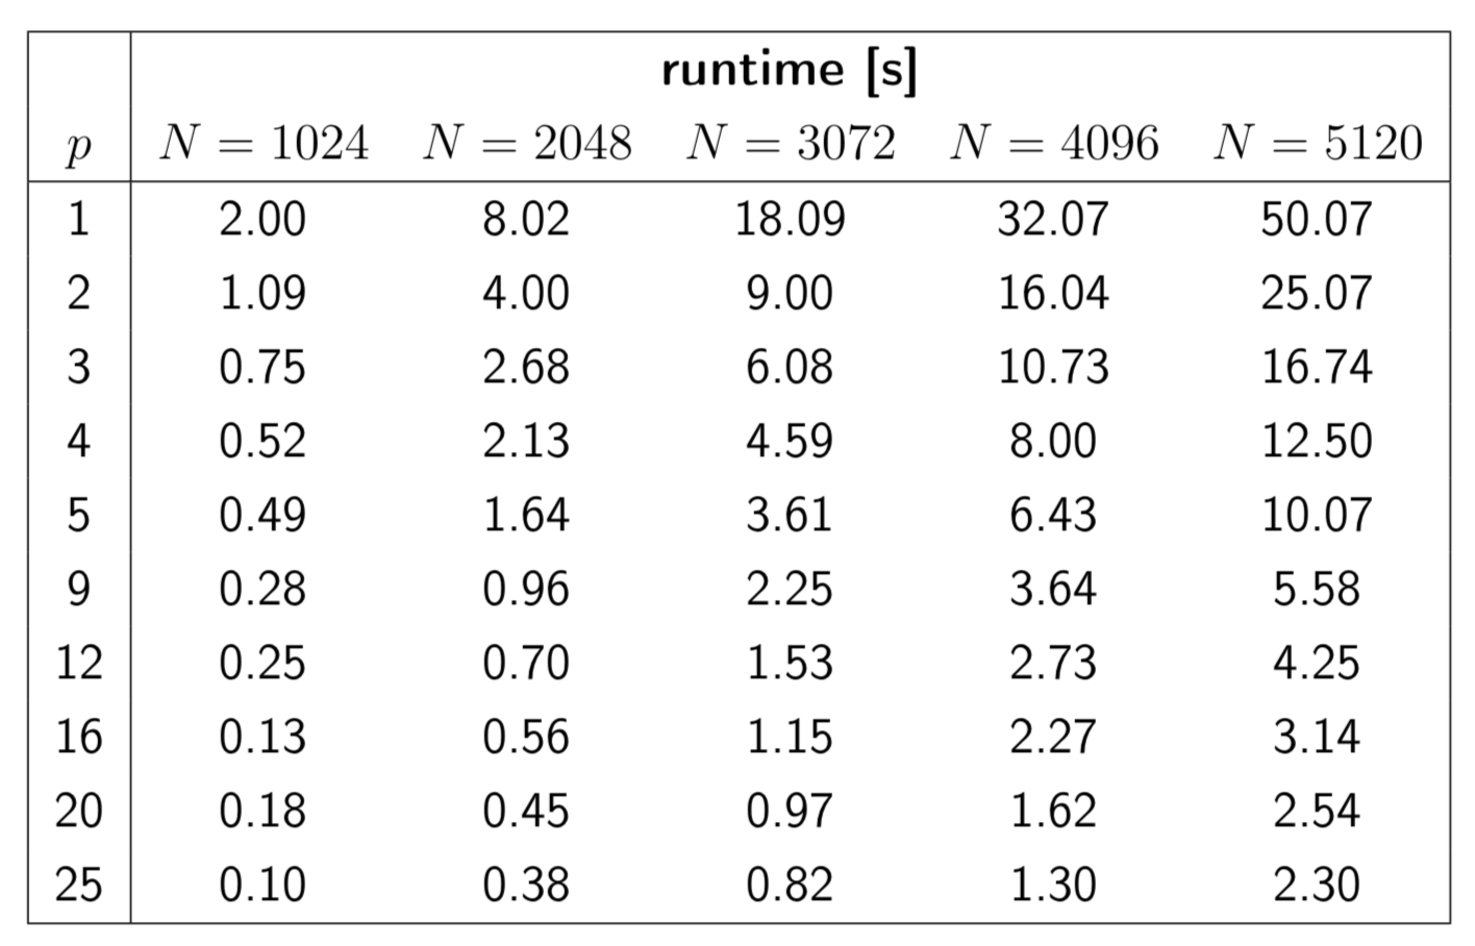
\includegraphics[scale=0.5]{fig2.pdf} 
    \end{center}
    \caption{Given hypothetical data for weak scaling analysis.} 
    \label{fig:2}
\end{figure}

\begin{figure}[hb!]
    \begin{center}
    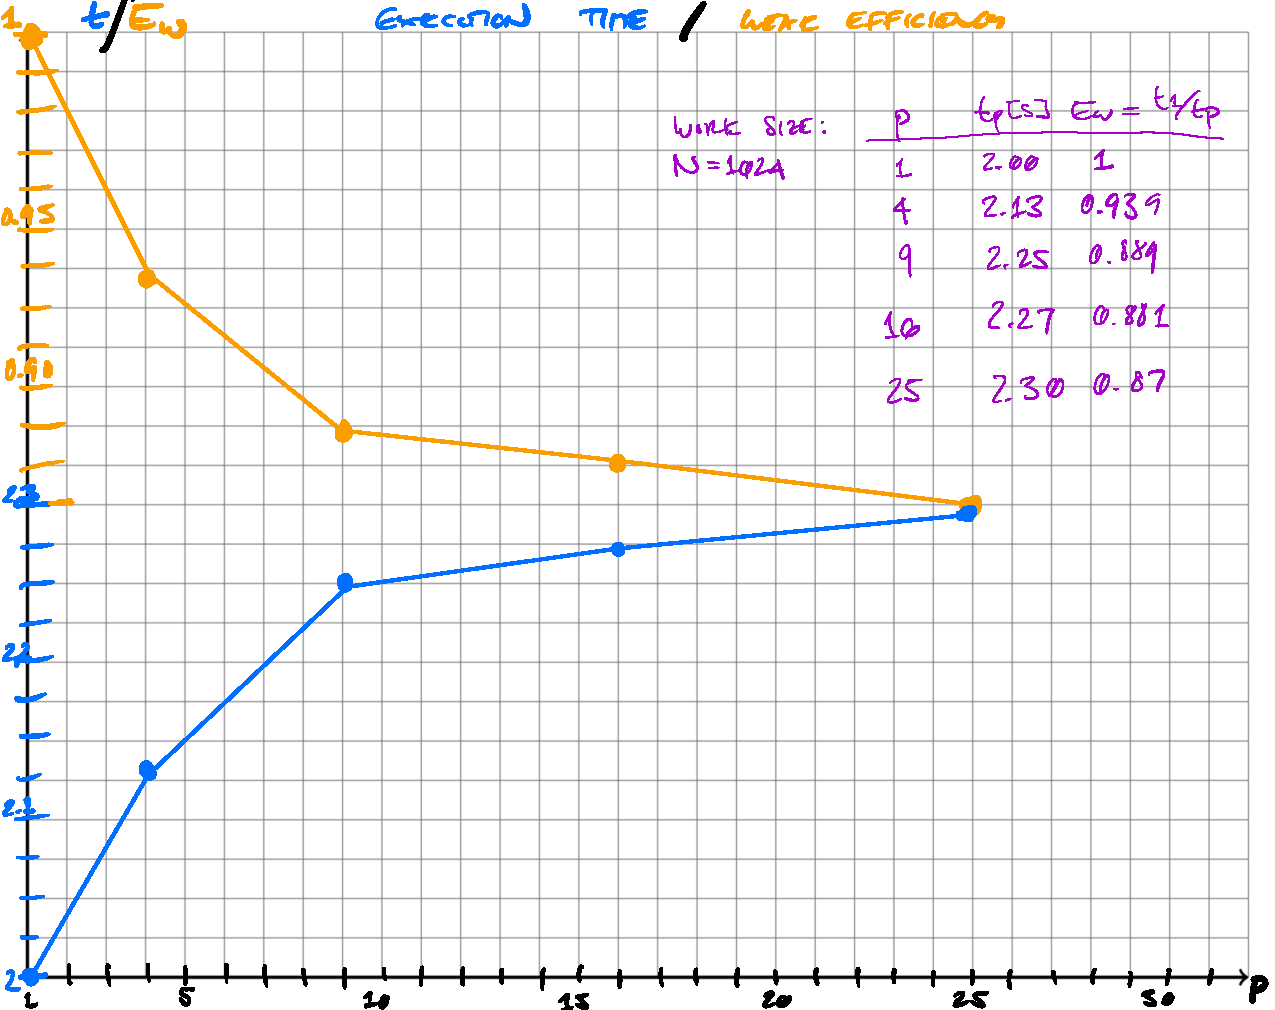
\includegraphics[scale=0.7]{fig3.pdf} 
    \end{center}
    \caption{Hypothetical data weak scaling plot for $N=1024,\ p=1$ as baseline reference.} 
    \label{fig:3}
\end{figure}

\end{document}